\documentclass{standalone}

\usepackage{tikz}

\begin{document}
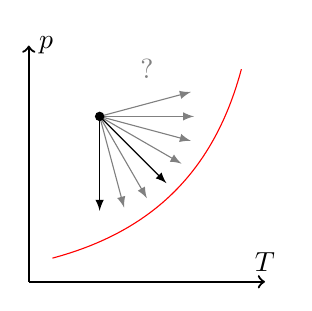
\begin{tikzpicture}[x=3cm, y=3cm]
  % Axis
  \draw[->, thick] (0,0) -- (0,1) node[right] {$p$};
  \draw[->, thick] (0,0) -- (1,0) node[above] {$T$};

  % Saturation curve
  \draw[red] (0.1, 0.1) to[bend right=30] (0.9,0.9);

  % Arrows
  \draw[-latex, gray] (0.3, 0.7) -- ++(-75:0.4);
  \draw[-latex, gray] (0.3, 0.7) -- ++(-60:0.4);
  \draw[-latex, gray] (0.3, 0.7) -- ++(-30:0.4);
  \draw[-latex, gray] (0.3, 0.7) -- ++(-15:0.4);
  \draw[-latex, gray] (0.3, 0.7) -- ++(  0:0.4);
  \draw[-latex, gray] (0.3, 0.7) -- ++( 15:0.4);
  \node[gray] at (0.5,0.9) {?};

  \draw[-latex] (0.3, 0.7) -- ++(-45:0.4);
  \draw[-latex] (0.3, 0.7) -- ++(-90:0.4);

  % Starting point
  \fill (0.3,0.7) circle (0.02);
\end{tikzpicture}
\end{document}
